\documentclass[11pt, fleqn]{article}

\usepackage{../../mainStructure}
\usepackage{relsize,exscale}

\begin{document}
	\title{Classical \& Quantum Solitons\\
	\large{Based on a Course Given by Nick Manton}}
	\author{Notes by Sam Crawford}
	\maketitle

\tableofcontents

\section{Kinks}

\subsection{Kinks in $ \phi^4 $ theory}

\todo[inline]{Intro, mention the fact we're working in $ 1+1 $D}

\paragraph{} We begin with the relativistic Lagrangian density for a real scalar field
	\begin{equation}\label{key}
		\mathcal{L} = \tfrac{1}{2} \partial_\mu \phi \partial^\mu \phi - U(\phi) .
	\end{equation}
Varying this yields the standard Euler-Lagrange equations of motion to be
	\begin{equation}\label{eq:scalarField}
		\partial_\mu \partial^\mu \phi + \frac{d U}{d \phi} = 0.
	\end{equation}
Note that in the case $ U(\phi) = \tfrac{1}{2} m^2 \phi^2 $, this is just the Klein-Gordon equation. However, we are instead interested in the class of solutions that occur when the potential $ U $ has multiple distinct minima, which we will refer to as \textbf{vacua}. In $ \phi^4 $ theory, we use the potential $ U(\phi) = \tfrac{1}{2} (1 - \phi^2)^2 $:

\begin{center}
	\begin{tikzpicture}

      \draw[->] (-3,0) -- (4.2,0) node[right] {$\phi$};
      \draw[->] (0,-0.2) -- (0,4.2) node[above] {$U(\phi)$};
     \draw[scale=0.5,domain=-2.25:2.25,smooth,variable=\x] plot ( {2*\x} , {0.5* (1-\x*\x)^2} );
      
\node [below] at (-1,0) {$-1$};
\node [below] at (1,0) {$1$};
\end{tikzpicture}
\end{center}

The two vacua here are $ \phi = \pm 1 $, where the potential energy vanishes. We can find \textit{static} solutions to this theory by setting $ \dot{\phi} \equiv 0 $, whence the equations of `motion' become
	\begin{equation}\label{key}
		-\phi '' + 2 \phi (1- \phi^2) = 0.
	\end{equation}
Specifically, we shall look for static solutions which \textit{connect} the vacua. In this example with one spatial dimension, this means that we impose the boundary conditions
	\begin{equation}\label{key}
		\lim_{x \to \pm \infty} \phi(x) = \pm 1.
	\end{equation}
\paragraph{} We can find solutions of this form by considering the \textit{energy} associated to a given field configuration, which arises in typical Noetherian fashion from the time-translational symmetry of the Lagrangian. This energy functional is
	\begin{equation}\label{eq:phi4energy}
		E [ \phi ] = \int_\mathbb{R} \left( \tfrac{1}{2} \dot{\phi}^2 + \tfrac{1}{2} \phi '^2 + U(\phi) \right) \mathrm{d}x.
	\end{equation}
For completeness, we still have the $ \dot{\phi} $ term present in this functional, though in our search for static solutions this shall be set to $ 0 $. It is important to notice that, whilst this looks very similar to the \textit{action} functional that arises from integrating the Lagrangian density, it is a separate entity, most notably due to the fact that the integral is taken over the \textit{spatial} dimension rather than over time.

\paragraph{} The following method of minimising the energy of a static field configuration is due to Bogomolny, and will appear throughout this course. It involves `completing the square' for the energy functional, then interpreting the resulting terms. As $ U \geq 0 $ for this potential, it is fairly easy to guarantee the existence of a function $ W(\phi) $ satisfying
	\begin{equation}\label{key}
		U(\phi) = \frac{1}{2} \left( - \frac{d W}{d \phi} \right)^2.
	\end{equation}

From here we write
	\begin{align*}
		E
		&= \frac{1}{2} \mathop{\mathlarger{\int}}_\mathbb{R} \Bigg( \phi'^2 + \left( \frac{d W}{d \phi} \right)^2 \Bigg) \mathrm{d} x, \\
		&= 	\frac{1}{2} \mathop{\mathlarger{\int}}_\mathbb{R} \left( \phi' \mp \left( \frac{d W}{d \phi} \right) \right)^2 \mathrm{d}x
		\pm \mathop{\mathlarger{\int}}_\mathbb{R} \frac{dW}{d \phi} \frac{d \phi}{dx} \mathrm{d}x.
 	\end{align*}
We then note that the last term is a total derivative, and hence depends only on the values of $ W $ on the boundary conditions on $ \phi $. The fact that this boundary term does not vanish in general is what gives rise to the notion that the solutions generated are \textit{topological} in nature, as no amount of smooth deformation within the finite $ x $ region can lead to a change in this boundary term. Note further that the integrand of the first term is positive everywhere, this can be used to determine a lower bound, the \textbf{Bogomolny bound} of the energy\footnote{Note the $ \pm $, if our boundary term turned out to be negative, we could exploit the sign ambiguity in determining $ W $ to ensure that our lower bound for the energy is always positive.}
	\begin{equation}\label{key}
		E \geq \pm \left[ W ( \phi ( + \infty)) - W ( \phi ( - \infty)) \right].
	\end{equation}
Moreover, we can write down the condition for this energy bound to be saturated (i.e. for $ \geq $ to become $ = $ ), known as the \textbf{Bogomolny equation}
	\begin{equation}\label{key}
		\phi' = \pm \frac{d W}{d \phi}.
	\end{equation}

\paragraph{} So far this discussion has been a bit general. In the case of $ \phi^4 $, it is fairly easy to show that
	\begin{equation}
		W(\phi) = \phi - \frac{1}{3} \phi^3
	\end{equation}
is the desired function. Imposing our boundary conditions we see that $ W(\phi(\pm \infty)) = \pm \nicefrac{2}{3} $. The solution of the resulting Bogomolny equation, $ \phi' = 1 - \phi^2 $, is the \textit{kink} solution 
\begin{equation}
	\phi(x) = \tanh (x-a).
\end{equation}
We call the Bogomolny energy of this solution the \textit{mass} of the kink, which is $ {M = \nicefrac{4}{3}} $.  This is a family of solutions parametrised by the location at which the kink crosses the $ x $-axis. Understanding the degrees of freedom in our solutions will be a common theme, and we refer to the space of such parameters as the \textbf{moduli space} for the solutions, which in this case is simply $ \mathbb{R} $.

\paragraph{} As $ \phi^4 $ is a relativistic theory, from here we can obtain a family of dynamic solutions by considering Lorentz boosts of our static one. Applying a boost of speed $ v $ we obtain
	\begin{equation}\label{eq:phi4kink}
		\phi(x,t) = \tanh\left[ \gamma ( x - vt - a ) \right].
	\end{equation}
However, we can also find a family of \textit{approximate} solutions by allowing our position in the moduli space to vary over time. Whilst this may seem pointless in this case, it is a strategy that will prove far more tractable for higher-dimensional solitons. So, we begin with the ansatz $ \phi(x,t) = \tanh(x - a(t)) \Rightarrow \dot{\phi} = -\dot{a}\phi' $, and consider the `kinetic' term in \eqref{eq:phi4energy}, which we find to be
	\begin{equation}\label{key}
		T = \frac{1}{2} \int_\mathbb{R} \dot{\phi}^2 \mathrm{d}x = \frac{1}{2} \dot{a}^2 \int_\mathbb{R} \phi'^2 \mathrm{d}x = \frac{1}{2} M \dot{a}^2.
	\end{equation}
Note that, as we are only varying the parameter specifying static solutions, we have by necessity a constant potential energy $ V = M $. Hence we can write an effective Lagrangian in moduli space as
	\begin{equation}\label{key}
		\mathscr{L} = \frac{1}{2} M \dot{a}^2 - M.
	\end{equation}
Varying $ a $ then leads to the effective equation of motion $ M \ddot{a} = 0 $. We can think of this as an equation for finding \textit{geodesics} in the moduli space, which in this case turn out to simply be straight lines. Solutions of this naturally have the form $ a(t) = vt + c $, thus we have an equation very similar to \eqref{eq:phi4kink}, though without the relativistic dilation due to the $ \gamma $ factor. This approximation thus becomes more accurate when $ v \ll 1 $.

\subsection{Quantisation of Kink Motion}

\paragraph{} By employing the approximate solutions obtained from the moduli space, we can attempt canonical quantisation of $ \phi^4 $ theory easily, as we have then reduced our consideration to just one degree of freedom. First, consider the canonically conjugate momentum of $ a $
	\begin{equation}\label{key}
		P = \frac{\partial \mathscr{L}}{\partial \dot{a}} = M \dot{a}.
	\end{equation}
Upon quantisation, this is then promoted to the linear operator $ \hat{P} = -i \hbar \frac{\partial}{\partial a} $. Dropping the constant $ M $ from the Hamiltonian, we then have
\begin{equation}\label{key}
	\hat{H} = \frac{\hbar^2}{2M} \frac{\partial^2}{\partial a^2}.
\end{equation}
We then have a set of plane wave eigenstates $ \langle a | k \rangle = \psi(a) \propto e^{ika} $.

\subsection{The Sine-Gordon Model}

\paragraph{} The sine-Gordon model\footnote{Yes, the name is a pun on Klein-Gordon...} is similar to $ \phi^4 $, in that it simply involves changing the potential function to $ U(\phi) = 1 - \cos \phi $. Now we have an infinite number of vacua, each separated by $ 2 \pi $. We shall learn however that we can only find static solutions which connect \textit{adjacent} vacua, a result which in fact has a physical interpretation as a consequence of sine-Gordon solitons `interacting'.

\paragraph{} As we have a discrete symmetry of the form $ \phi \to \phi + 2 \pi n $, we can also consider the quotient space $ \phi : \mathbb{R}^{1,1} \to \mathbb{R}/\mathbb{Z} \simeq S^1 $. Now we have a single vacuum, however the field is no longer linear. We can also consider compactifying the $ x $-axis, to obtain the space $ S^1_\infty \simeq \mathbb{R} \cup \{ \infty \} $. Hence we have a map between two circles, which has a natural topological invariant: the \textit{winding number}. There are three different ways we might define this:
	\begin{itemize}
		\item [(Na\"ive)] We could discar all notions of circles and return to maps from $ \mathbb{R} \to \mathbb{R} $. In order to have a finite energy, our solutions must be subject to boundary conditions	
			\begin{equation}\label{key}
				\lim_{x \to \pm \infty} \phi (x) = 2 \pi n_\pm.
			\end{equation}
		The \textbf{topological charge} would then be $ Q = n_+ - n_- $, which naturally must be conserved due to the fact that $ Q $ must be an integer, yet can may only be deformed in a continuous manner by the evolution of the field theory.
		
		\item[(Physics)] One can show that \textit{any} configuration of the field, including those which do not satisfy the equations of motion, must conserve the current
			\begin{equation}\label{key}
				j^\mu = \frac{1}{2 \pi} \epsilon^{\mu\nu} \partial_\nu \phi = \frac{1}{2 \pi} (\partial_x \phi, - \partial_t \phi).
			\end{equation}
		Computing $ \partial_\mu j^\mu $ then shows this vanishes trivially. The topological charge is then the associated conserved quantity $ Q = \int j^0 \mathrm{d}x = \int \mathrm{d}\phi = n_+ - n_- $.
		
		\item[(Geometry)] In differential geometry, the degree of a mapping $ \phi: S^1_\infty \to S^1 $ is determined by selecting a volume form on $ S^1 $, in this case $ \mathrm{Vol} = \tfrac{1}{2 \pi} d\phi $ which is normalised such that $ \int_{S^1} \mathrm{Vol} = 1 $. This is then pulled back to the source space via the map, i.e. $ \mathrm{Vol}_{S^1_\infty} = \phi^* \mathrm{Vol} = \tfrac{1}{2 \pi} \tfrac{\partial \phi}{\partial x} dx$. Integrating this over the source space $ S^1_\infty $ then defines $ Q $, which arises from the same integral as in the physical consideration.
	\end{itemize}

\paragraph{} To find static sine-Gordon kinks we can again utilise the Bogomolny method, this time with the function
	\begin{equation}\label{key}
		W(\phi) = \pm \cos \left( \tfrac{1}{2} \phi \right).
	\end{equation}
Which leads to the Bogomolny equation
	\begin{equation}\label{key}
		\phi(x) = 4 \tan^{-1} e^{(x-a)}.
	\end{equation}
	
\paragraph{} Not only does the sine-Gordon model exhibit soliton solutions, it is also an example of an \textit{integrable system}. It admits solutions containing multiple solitons, which can collide and interact in a non-linear manner yet still emerge asymptotically `unchanged'. Finding exact expressions for $ N $-kink solutions is always possible in principle, but quickly requires disgusting levels of algebraic manipulation. The $ Q = 2 $ solution is
	\begin{equation}\label{key}
		\phi(x,t) = 4 \tan^{-1}\left( \frac{v \sinh \gamma x}{\cosh \gamma v t} \right).
	\end{equation}
The fact that this looks like two well separated kinks approaching, then repelling one another is not immediately obvious. Never the less this is what we see if the function is plotted. In general, by using similar moduli space arguments as we did previously, one can show that kinks `repel' other kinks and `attract' anti-kinks.\todo{Show}

\section{Vortices}

\subsection{The Abelian Higgs Model}

\paragraph{} We shall now move up to $ 2 + 1 $ dimensions. It is rare to find vortices in real scalar field theories, thus we shall usually consider other classes of theories. Our first example, the Abelian Higgs model, has a $ U(1) $ gauge field coupled to a complex scalar field via the Lagrangian
	\begin{equation}\label{key}
		\mathcal{L} = -\frac{1}{4} F^{\mu\nu}F_{\mu\nu} + \frac{1}{2}\left( D_\mu \varphi \right)^* \left( D^\mu \varphi \right) - \frac{\lambda}{8} (1 - |\varphi| )^2.
	\end{equation}
By varying each of the fields, we obtain the equations of motion
	\begin{align}
		\partial_\mu F^{\mu\nu} &= \frac{i}{2} \left( ( D^\nu \varphi)^* \varphi - \varphi^* (D^\nu \varphi) \right),\\
		D_\mu D^\mu \varphi		&= \frac{\lambda}{2} \varphi (1 - |\varphi|^2).
	\end{align}

\paragraph{} Obtaining the energy functional for the Abelian Higgs model is a little more involved. However, after some work, we can obtain the \textbf{Ginzburg-Landau energy}
	\begin{equation}\label{eq:Ginzburg}
		E[\varphi] = \int_{\mathbb{R}^2} \left\{ \frac{1}{2} B^2 + \frac{1}{2} (D_1 \varphi)^*(D_1 \varphi) + (D_2 \varphi)^*(D_2 \varphi) + \frac{\lambda}{8} (1 - |\varphi|)^2 \right\} \mathrm{d}^2x,
	\end{equation}
where $ B $ is the magnetic field strength $ B = F_{12} = \partial_1 A_2 - \partial_2 A_1 $.

\paragraph{} This model has some physical relevance when attempting to model planar superconductors. By varying the parameter $ \lambda $, we can make vortices attract ($ \lambda > 1 $) or repel ($ \lambda < 1 $), these are respectively referred to as \textit{type I/II behaviour}. In order to use the Bogomolny method, we choose to take the \textit{critical copuling} value, $ \lambda = 1 $.

\paragraph{} When studying the Abelian Higgs model, it is convenient to work in polar coordinates. Firstly, we shall write down the relevant terms in a basis-invariant manner. The gauge field $ A^\mu $ is in fact the one form 
	\begin{equation}\label{eq:A1Form}
		A = A_0 dt + A_1 dx^1 + A_2 dx^2.
	\end{equation}
The field strength $ F^{\mu\nu} $ can then be written as the $ 2 $-form $ F = dA $, where $ d $ denotes the exterior derivative of a differential form. A basis vector for the space of $ 2 $-forms can be written $ dx^\mu \wedge dx^\nu $ where, to prevent overcounting, we assume $ \mu < \nu $. To transform into polar coordinates, we write
	\begin{equation}\label{key}
		x = r \cos \theta, \quad y = r \sin \theta.
	\end{equation}
We obtain the transformation between $ 1 $-forms by differentiating this relation:
	\begin{equation}\label{key}
		dx = dr \cos \theta - r \sin \theta d \theta, \quad dy = dr \sin \theta + r \cos \theta d \theta.
	\end{equation}
We then substitute this into \eqref{eq:A1Form} and collect coefficients to obtain
	\begin{equation}\label{key}
		A = \underbrace{(A_1 \cos \theta + A_2 \sin \theta)}_{\eqqcolon A_r} dr + \underbrace{r(A_2 \cos \theta - A_1 \sin \theta)}_{\eqqcolon A_\theta} d\theta.
	\end{equation}
	
\subsection{Vortices \& Topology}

\paragraph{} Recall that the potential term for the Abelian Higgs (disregarding the gauge field) is $ U(\varphi) = (1 - |\varphi|)^2 $. Thus the vacuum for this theory is the connected space $ \{ \varphi : |\varphi|^2 = 1 \} \simeq S^1 $. To find finite energy solutions, we impose the boundary conditions $ |\varphi| \to \infty $, $ B \to 0 $ and $ D \varphi \to 0 $ as $ |\mathbf{x}| \to \infty $. We can then apply gauge fixing conditions, which result in the existence of a function $ \mathcal{X} (\theta) $ such that
	\begin{equation}\label{key}
		\lim_{r \to \infty} \varphi(r,\theta) = e^{i \mathcal{X}(\theta)}.
	\end{equation}
For compatibility, as $ \varphi(r, \theta) = \varphi(r, \theta + 2\pi) $, we must have that $ \mathcal{X}(\theta + 2\pi) = \mathcal{X}(\theta) + 2 \pi N $. We then refer to $ N $ as the winding number of the field configuration. This number is invariant under gauge transformation, field transformations and time evolution, thus it is a topological charge.

\paragraph{} There is a physical interpretation of this charge. Consider the boundary condition $ D_\theta \varphi \to 0 $. If we define $ \tilde{A}_\theta (\theta) \coloneqq \lim_{r \to \infty} A_\theta(r,\theta) $, then this can implies
	\begin{equation}\label{eq:AThetaLim}
		\partial_\theta e^{i \mathcal{X}(\theta)} - i \tilde{A}_\theta (\theta) e^{i \mathcal{X}(\theta)} = i \left( \mathcal{X}'(\theta) - \tilde{A}_\theta(\theta) \right) e^{i\mathcal{X}(\theta)} = 0.
	\end{equation}
The \textbf{magnetic flux} is defined as
	\begin{equation}\label{key}
		\Phi \coloneqq \int_{\mathbb{R}^2} B \; \mathrm{d}^2x = \int_\mathbb{R} \mathrm{d}r \int_{S^1} \mathrm{d}\theta \, F_{r\theta}.
	\end{equation}
This can be simplified by noting that $ \int_{S^1} \left( \partial_\theta A_r \right) \mathrm{d}\theta = 0 $ as we have a total derivative and $ S^1 $ has no boundary. Similarly, when considering the $ A_\theta $ term, we have a total derivative in $ r $, ignoring the `boundary' at $ r = 0 $,\footnote{Technically, we are considering the integral over the finite region $ \overline{B_r} = \{ \mathbf{x} \in \mathbb{R}^2 : x \leq r \} $, and employing Stoke's theorem: $ \int_M d\omega = \int_{\partial M} \omega $ and taking the limit as $ r \to \infty $. } we thus have
	\begin{equation}\label{key}
		\Phi = \int_{S^1} \tilde{A}_\theta \, \mathrm{d}\theta.
	\end{equation}
From \eqref{eq:AThetaLim}, we know this is also a total derivative
	\begin{equation}\label{key}
		\Phi = \int_0^{2 \pi} \mathcal{X}'(\theta) \, \mathrm{d}\theta = \mathcal{X}(2\pi) - \mathcal{X}(0) = 2 \pi N.
	\end{equation}
	
\paragraph{} There is one more way we can obtain $ N $. In a move reminiscent of the analysis of complex function, we can draw a \textit{Jordan curve}\todo{Define?}{} in the plane, and consider the \textit{zeroes} of $ \varphi $ contained within. In the simple case that we enclose just one zero, whilst winding around it, we know that $ \arg \varphi $ must change by some integer multiple of $ 2 \pi $. If this multiple is $ \pm 1 $, we call the zero a \textbf{simple vortex} (or \textit{anti}-vortex, for $ n < 0 $). One can then show that if the set of zeroes, $ \{ \mathbf{x}_i \} $, have multiplicity $ n_i $, then the overall winding around the curve is $ N = \sum_i n_i $. To interpret $ N $ as the topological charge, we then simply consider the case that the Jordan curve is sufficiently large to enclose all the zeroes of $ \varphi $. If we think of the simple zeroes as (anti-)vortices, then non-simple zeroes are to be interpreted as the superposition of multiple vortices, each of which `carries' a flux of $ \pm 2 \pi $.

\subsection{The Basic Vortex}

\paragraph{} To find a simple vortex solution. We impose the same boundary conditions as before, and further require that $ N = 1 $, and search for static solutions which minimize the Ginzburg-Landau energy \eqref{eq:Ginzburg}. Let's try the ansatz
	\begin{subequations}\begin{align}
		A_r(r, \theta) &= 0, \\
		A_\theta(r, \theta) &= f(r), \\
		\varphi (r,\theta) &= h(r) e^{i\theta}.
	\end{align}\end{subequations}
This form for $ A $ is known as \textbf{radial gauge}. The equations of motion then become
	\begin{align}
		\frac{d^2 h}{dr^2} + \frac{1}{r} \frac{dh}{dr} - \frac{1}{r^2} (1-f)^2 h + \frac{\lambda}{2} (1 - h^2) h &= 0,\\
		\frac{d^2 f}{dr^2} - \frac{1}{r} \frac{d f}{dr} + (1-f) h^2 &= 0.
	\end{align}
Unfortunately, only \arabic{page} pages into the course and we have already encountered our first system of equation for which we do not have analytical solutions. We must resort to numerical methods\todo{Reference?}. A sketch of the solution for $ f $ and $ h $ looks something like
	\begin{center}
		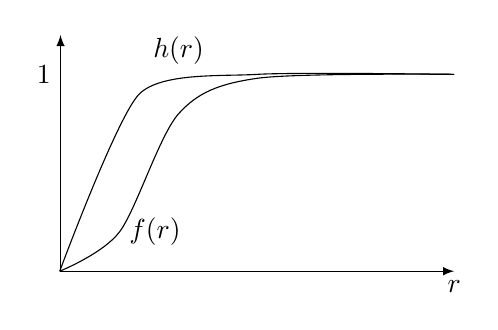
\begin{tikzpicture}

\draw [-latex] (0,-0.01) -- (0,3) ;
\draw [-latex] (-0.01,0) node (v1) {} -- (5,0);

\node (v3) at (2.5,2.5) {};
\node (v2) at (1,2.25) {};
\draw  plot[smooth, tension=0.4] coordinates {(v1) (v2) (v3) (5,2.5) };
\node [right] (v4) at (0.75,0.5) {$f(r)$};
\draw  plot[smooth, tension=.5] coordinates {(v1) (0.75,0.5) (1.5,2) (2.5,2.45) (5,2.5) };

\node at (1.5,2) {};
\node (v5) at (5,2.5) {};
\node [below] at (5,0) {$r$};
\node [above] at (1.5,2.5) {$h(r)$};
\node [left] at (0,2.5) {$1$};
\end{tikzpicture}
	\end{center}

\subsection{Bogomolny Equations for Vortices}\label{sec:BogoVort}

We can attempt to complete the square of \eqref{eq:Ginzburg} without defining any new functions. To begin, we write
	\begin{align}
		\begin{split}
			E = \frac{1}{2} \int_{\mathbb{R}^2} \left\{ \left( B - \tfrac{1}{2} (1 - |\varphi|^2) \right)^2 + \left( D_1 \varphi + i D_2 \varphi \right)^* \left( D_1 \varphi + i D_2 \varphi \right) \right\} \mathrm{d}^2x\\
			+ \frac{1}{2} \int_{\mathbb{R}^2} \left\{ B(1 - |\varphi|^2)^{\phantom 2 } +i \left( \left( D_2 \varphi \right)^* D_1 \varphi - \left(D_1 \varphi\right)^* D_2 \varphi \right)  \right\} \mathrm{d}^2x.
		\end{split}
	\end{align}
Whilst this looks far less helpful, we can simplify it by making use of the identities
	\begin{subequations}\begin{align}
		\partial_2 \left( \varphi^* D_1 \varphi \right) &\equiv \left( D_2 \varphi \right)^* D_1 \varphi + \varphi^* D_2 D_1 \varphi, \\
		(D_1 D_2 - D_2 D_1) \varphi &\equiv -iB\varphi.
	\end{align}\end{subequations}
With these, the second integral becomes
	\begin{equation*}\label{key}
		\frac{1}{2} \int_{\mathbb{R}^2} B \, \mathrm{d}^2x + \frac{i}{2} \int_{\mathbb{R}^2} \left\{ \partial_2 \left( \varphi^* D_1 \varphi \right) - \partial_1 \left( \varphi^* D_2 \varphi \right) \right\} \, \mathrm{d}^2x .
	\end{equation*}
The first term of this is simply the magnetic flux, and the second term is a pair of total derivatives, which vanish according to our boundary conditions. Hence, our energy can be written
	\begin{equation}\label{key}
		E = \frac{1}{2} \int_{\mathbb{R}^2} \left\{ \left[ B - \tfrac{1}{2}(1-|\varphi|) \right] ^2 + \left| D_1 \varphi + i D_2 \varphi \right|^2 \right\} \, \mathrm{d}^2x + \pi N.
	\end{equation}
Thus we get the Bogomolny bound $ E \geq \pi N $,\footnote{Assuming $ N > 0 $, if this is not the case, as before we simply need to flip some signs when completing the square.} which is saturated by solving the Bogomolny equations
	\begin{subequations}\begin{align}
		D_1 \varphi + i D_2 \varphi &= 0, \label{eq:vortexBogo1} \\
		B - \tfrac{1}{2} (1-|\varphi|^2) &= 0. \label{eq:vortexBogo2}
	\end{align}\end{subequations}

\paragraph{} Whilst unfortunately we still cannot find analytical solutions to these equations, we can at least reduce them to an equation in a single scalar variable as follows: If we define the function $ \rho $ to be such that $ \varphi = e^{\tfrac{\rho}{2} + i\mathcal{X} } $, then \eqref{eq:vortexBogo1} implies that $ B = -\tfrac{1}{2} \Delta \rho $. Substituting this into \eqref{eq:vortexBogo2}, we might then na\"ively write
	\begin{equation}\label{key}
		\Delta \rho - e^\rho + 1 = 0.
	\end{equation}
However, we have failed to account for the behaviour of $ \rho $ around the zeroes of $ \varphi $. We can analyse the behaviour of $ \varphi $ asymptotically as it approaches a zero located at $ \mathbf{x}_i $, in which case we find
	\begin{subequations}
			\begin{align}
						|\varphi| 		&\sim | \mathbf{x} - \mathbf{x}_i |, \\
				\Rightarrow \phantom{a} \rho 	&\sim 2 \log | \mathbf{x} - \mathbf{x}_i |, \label{eq:rhoSingularity} \\
				\Rightarrow \Delta\rho &\sim 4 \pi \delta^{(2)} (\mathbf{x} - \mathbf{x}_i ).
			\end{align}
	\end{subequations}
Ignoring \eqref{eq:rhoSingularity} as it is comparatively negligible, we then arrive at \textbf{Taube's equation}
	\begin{equation}\label{eq:Taube}
		\Delta \rho - e^\rho + 1 = 4 \pi \sum_{i=1}^N \delta^{(2)} ( \textbf{x} - \textbf{x}_i ) .
	\end{equation}
Even without finding its solutions, Taube's equation can tell us a lot about vortex solutions. Given the boundary condition, $ \rho \to 0 $ as $ | \mathbf{x} | \to \infty $, we have unique solutions for any given set of points $ \{ \mathbf{x}_i \} $. This gives us a \textit{moduli space} for $ N $-vortex solutions. Note, this space is \textit{not} simply $ \mathbb{R}^{2N} $, as we have a redundancy in exchanging $ \mathbf{x}_i $ with $ \mathbf{x}_j $. Later we shall see how we can better describe this moduli space, through complex polynomials, of all things.

\subsection{Properties of Bogomolny Vortices}

\paragraph{} What does a vortex `look like'? Recall \eqref{eq:vortexBogo2}, and consider the centre of the vortex, where $ \varphi = 0 $. Here we have $ B = \nicefrac{1}{2} $, and if we assume this to be roughly constant, the fact that each vortex contributes a flux of $ 2 \pi $ means that $ \Phi = 2 \pi \approx B \cdot A $, thus the `area' of the vortex is roughly $ 4 \pi $, i.e. its radius is roughly $ 2 $.

\paragraph{} To gain more of an insight, we should return to our analysis of $ \rho $. As we already established, $ \rho $ heads to $ -\infty $ logarithmically as we head towards a zero of $ \varphi $. But when we head away from a zero, as $ |\varphi| \to 1 $ we must have that $ \rho \to 0 $, which means we can consider the linearisation of Taube's equation
	\begin{equation}\label{key}
		\Delta \rho - \rho = 0 + \mathcal{O}\left( \rho^2 \right).
	\end{equation}
If we assume that this approximation is accurate at the maxima of $ \rho $, which is reasonable, as we would expect maxima to occur far away from zeroes, then $ \Delta \rho \leq 0 \Rightarrow \rho \leq 0 $. Hence, everywhere $ \rho \leq 0 $ which, in terms of the observable vortex properties, means that $ |\varphi| \leq 0 $, $ B \geq 0 $.

\todo[inline]{Plot stuff with $ \rho $}

\subsection{Moduli Space of Vortex Solutions}

\paragraph{}Recall that in \cref{sec:BogoVort} we discovered a way of parametrising vortices via the unique solutions of Taube's equation \eqref{eq:Taube}. We'll now turn to the problem of understanding the space in which these solutions lie, which we shall call $ M_N $ in the case of $ N $-vortex solutions. As we are in 2$ D $, we can make the identification $ \mathbb{R}^2 \simeq \mathbb{C} $ by setting $ z \coloneqq x^1 + i x^2 $. Letting $ z_i $ denote the complex locations of the zeroes of $ \varphi $ we can define a polynomial
	\begin{equation}\label{eq:cplxPolyFactor}
		P(z) = (z-z_1)(z-z_2)\cdots(z-z_N).
	\end{equation}
This gives us a function which is \textit{different} from the Higgs field $ \varphi $, though it does have the same zeroes. Considering the space of degree $ N $ complex polynomials, we see that \textit{this} is the same as the moduli space of $ N $-vortex solutions, as interchanging any pair of zeroes leaves the overall polynomial invariant, just as it leaves the vortex solution invariant. The reason any degree $ N $ polynomial works is the \textit{fundamental theorem of algebra}, which states that any polynomial of the form
	\begin{equation}\label{eq:cplxPolyLong}
		P(z) = z^N + a_{N-1} z^{N-1} + \cdots + a_1 z + a_0
	\end{equation}
has precisely $ N $ roots (accounting for multiplicity), and hence can be factorised into the form \eqref{eq:cplxPolyFactor}.

\paragraph{} There are a couple of ways we can conclude from here. Practically, we simply take the $ N $-tuple of complex coefficients $ (a_i)_{i=0}^{N-1} $ as the parametrisation of our complex space. However, one might then think that we have found a map $ \mathbb{C} \simeq \mathbb{R}^{2N} \to M_N $, and hence the moduli space \textit{is} just $ \mathbb{R}^{2N} $, right? But what is the geometry of the space of complex polynomials? If we let $ \mathbb{C}[z;N] $ denote the space of complex polynomials of degree \textit{at most} $ N $, we have to include lower degree polynomials in order for this space to have a vector structure. This space will also include polynomials for which $ a_N \neq 1 $, however, it is here that we notice a notion of equivalence. As we are only interested in the \textit{zeroes} of $ P(z) $, if we have a second polynomial $ Q(z) =  \lambda P(z) $, so long as $ \lambda \neq 0 $, these polynomials can be considered equivalent. If we quotient out by this equivalence relation, we can define the projective space of complex polynomials $ \mathbb{CP}[z;N] $. We can represent a point in this space by the set of coefficients, modulo scalar multiplication, which we write as $ [a_N, \cdots, a_0] $. In terms of moduli spaces, we have $ \mathbb{CP}[z;N] \simeq \cup_{i=1}^N M_i $, where the individual moduli spaces can be represented as $ M_i = \{ [ 0, \cdots, 1, a_{i-1}, \cdots, 0 ] \in \mathbb{CP}[z;N] \} $. This also allows us to understand the total moduli space as $ \mathbb{CP}[z] $, i.e. we remove the upper limit on the degree of polynomial.

\paragraph{} In summary, we can find a generic $ N $-vortex solution by selecting $ N $ complex numbers $ a_i $ to populate \eqref{eq:cplxPolyLong}, factorising this into the form \eqref{eq:cplxPolyFactor}, then substituting the resulting roots into Taube's equation \eqref{eq:Taube}. From here, we are guaranteed a unique solution $ \rho $, which in turn determines both $ \varphi $ and $ B $.

\todo[inline]{Vortex Scattering}

\subsection{Dynamics of Vortices}

\paragraph{} For solutions of the Abelian Higgs model which lie in $ M_N $, the effective Lagrangian is purely kinetic, as the potential energy is a constant $ \pi N $. This Lagrangian is
	\begin{equation}\label{key}
		\mathscr{L} = T = \tfrac{1}{2} \int_{\mathbb{R}^2}  \left( F_{0i}F_{0i} + \left( D_0 \varphi \right)^* D_0 \varphi \right) \mathrm{d}^2x.
	\end{equation}
Unlike last time, it is not so easy to write this directly in terms of the moduli space parameters $ a_i $, and in fact this integral is quite tricky to solve in general. We can however consider the special cases for $ N = 1,2 $. For the case of a single vortex with a center at $ z_1 = x^1_1 + i x^2_1 $, the kinetic term reduces to
	\begin{align}\label{eq:1Vortex}
		\mathcal{T} &= \frac{1}{2} \pi \left( \left( \frac{dx^1_1}{dt} \right)^2 + \left( \frac{dx^2_1}{dt} \right)^2 \right), \nonumber \\
		&= \pi \frac{dz_1}{dt} \frac{d \bar{z}_1}{dt}.
	\end{align}
As before, this it simply the line element of the Euclidean metric $ ds^2 = dz_1 d\bar{z}_1 = (dx^1_1)^2 + (dx^2_1)^2 $. Hence, just like the $ \phi^4 $ kinks, single vortex solutions travel along straight lines at a constant velocity.

\paragraph{} If we have two vortices, the polynomial for their zeroes is $ P(z) = (z-z_1)(z-z_2) = z^2 - (z_1 + z_2)z + (z_1 z_2)z $. Note that $ - a_1 = z_1 + z_2 $ corresponds to the `centre of mass' coordinate for the two vortices. It turns out in fact that this coordinate decouples from the system, and must simply solve a straight line equation such as \eqref{eq:1Vortex}. If we set $ a_1 \equiv 0 $, then $ z_2 \eqqcolon z = - z_1  $. We then have a reduced moduli space parametrised by $ a_0 = - z^2 \eqqcolon - b $, which we denote $ M^0_2 $. Again, the kinetic energy of the effective Lagrangian defines an equation for geodesics in $ M^0_2 $.

\section{Topology: Degrees of Mappings}

\section{Rational maps and the $ \sigma $-model}

\section{Skyrmions}

\end{document}